% questions.tex —— 1996 年·上海卷·理科 · 题目内容片段（无答案）
% 由 tools/generate_projects.py 依来源总账自 1996/1996_数学真题_上海理工农医_试题.md 生成，勿手改（改源 MD 后重跑）


\gkpart{数学试卷}

\begin{gktip}
\textbf{来源说明}：本题面依据固定来源 PDF 逐题转录。扫描件共 9 页，题面主要在第 1—4 页（印刷页码 74—77），第 24 题末尾续第 5 页；答案与评分解析自第 5 页起；第 9 页续有末题解析。原卷载明 24 道试题、满分 150 分，设 A1/B1、A2/B2 对应选做组；具体组别和计分规则按原卷保留。固定来源所载答案及评分解析另见答案要点、解析正文。来源出版者与官方性尚未核实；本稿待独立复核。

\textbf{图形说明}：第 7、8、18、20、21、23 题图形以 TikZ 按扫描件可辨认结构关系重绘；曲线比例和空间投影仅为示意，不作为额外数学条件。第 21 题另有评分解析中的辅助线示意。
\end{gktip}

\textbf{考生注意（按固定来源）：} 本试卷共有 24 道试题，满分 150 分。A1 组对应 B1 组，A2 组对应 B2 组。考生从对应的两组中可以且只可以选做一组；若同时做了对应的两组试题，或分别做了对应两组中的部分试题，则只对考生在 A 组中所完成的部分进行评分和计分。

\textbf{一、选择题（本大题满分 24 分，共 8 题，每题 3 分）}

每题有且只有一个正确结论，须把正确结论的代号写在题后的圆括号内；选对得 3 分，不选、选错或选出代号超过一个（不论是否都写在圆括号内），一律得零分。

\begin{question}
\gkti{1}已知集合

\nopagebreak[4]
\[
M=\{(x,y)\mid x+y=2\},\qquad N=\{(x,y)\mid x-y=4\},
\]

那么集合 $M\cap N$ 为\mbox{（　　）}。

（A）$x=3,\ y=-1$　　（B）$(3,-1)$　　（C）$\{3,-1\}$　　（D）$\{(3,-1)\}$

\end{question}
\begin{question}
\gkti{2}在下列各区间中，函数 $y=\sin\left(x+\dfrac{\pi}{4}\right)$ 的单调递增区间是\mbox{（　　）}。

（A）$\left[\dfrac{\pi}{2},\pi\right]$　　（B）$\left[0,\dfrac{\pi}{4}\right]$　　（C）$[-\pi,0]$　　（D）$\left[\dfrac{\pi}{4},\dfrac{\pi}{2}\right]$

\end{question}
\begin{question}
\gkti{3}如果 $\log_a3>\log_b3>0$，那么 $a,b$ 间的关系是\mbox{（　　）}。

（A）$0<a<b<1$　　（B）$1<a<b$　　（C）$0<b<a<1$　　（D）$1<b<a$

\end{question}
\begin{question}
\gkti{4}在下列命题中，真命题是\mbox{（　　）}。

（A）若直线 $m,n$ 都平行于平面 $\alpha$，则 $m\parallel n$。

（B）设 $\alpha-l-\beta$ 是直二面角，若直线 $m\perp l$，则 $m\perp\beta$。

（C）若直线 $m,n$ 在平面 $\alpha$ 内的射影依次是一个点和一条直线，且 $m\perp n$，则 $n$ 在 $\alpha$ 内或 $n$ 与 $\alpha$ 平行。

（D）设 $m,n$ 是异面直线，若 $m$ 与平面 $\alpha$ 平行，则 $n$ 与 $\alpha$ 相交。

\end{question}
\begin{question}
\gkti{5}将椭圆

\nopagebreak[4]
\[
\dfrac{x^2}{25}+\dfrac{y^2}{9}=1
\]

绕其左焦点按逆时针方向旋转 $90^\circ$ 后所得的椭圆方程是\mbox{（　　）}。

（A）$\dfrac{(x+4)^2}{25}+\dfrac{(y-4)^2}{9}=1$　　（B）$\dfrac{(x+4)^2}{25}+\dfrac{(y+4)^2}{9}=1$

（C）$\dfrac{(x+4)^2}{9}+\dfrac{(y-4)^2}{25}=1$　　（D）$\dfrac{(x+4)^2}{9}+\dfrac{(y+4)^2}{25}=1$

\end{question}
\begin{question}
\gkti{6}若函数 $f(x),g(x)$ 的定义域和值域都为 $\mathbb R$，则 $f(x)>g(x)\ (x\in\mathbb R)$ 成立的充要条件是\mbox{（　　）}。

（A）有一个 $x\in\mathbb R$，使得 $f(x)>g(x)$。

（B）有无穷多个 $x\in\mathbb R$，使得 $f(x)>g(x)$。

（C）对 $\mathbb R$ 中任意的 $x$，都有 $f(x)>g(x)+1$。

（D）$\mathbb R$ 中不存在 $x$，使得 $f(x)\le g(x)$。

\Needspace{0.4\textheight}
\end{question}
\begin{question}
\gkti{7}若 $\theta\in\left[0,\dfrac{\pi}{2}\right]$，则椭圆

\nopagebreak[4]
\[
x^2+2y^2-2\sqrt2x\cos\theta+4y\sin\theta=0
\]

的中心的轨迹是下列哪一幅图\mbox{（　　）}？
\nopagebreak[4]
\begin{center}% 固定来源 PDF 印刷页 74 第 7 题四组选项轨迹图的矢量示意。
% 四分之一椭圆弧仅表达原图所在象限及端点，不提供额外数据。
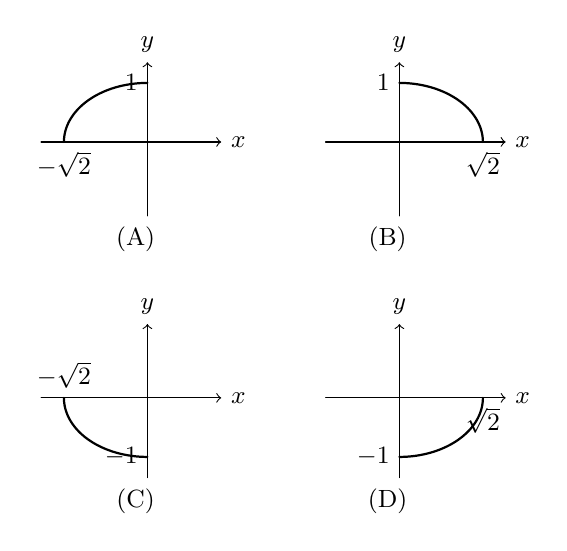
\begin{tikzpicture}[x=.75cm,y=.75cm,font=\small,line cap=round,line join=round]
  \begin{scope}
    \draw[->] (-1.8,0)--(1.25,0) node[right] {$x$};
    \draw[->] (0,-1.25)--(0,1.35) node[above] {$y$};
    \draw[thick,domain=0:90,samples=50] plot ({-1.414*cos(\x)},{sin(\x)});
    \node[below] at (-1.414,0) {$-\sqrt2$}; \node[left] at (0,1) {$1$};
    \node at (-.2,-1.65) {(A)};
  \end{scope}
  \begin{scope}[xshift=3.2cm]
    \draw[->] (-1.25,0)--(1.8,0) node[right] {$x$};
    \draw[->] (0,-1.25)--(0,1.35) node[above] {$y$};
    \draw[thick,domain=0:90,samples=50] plot ({1.414*sin(\x)},{cos(\x)});
    \node[below] at (1.414,0) {$\sqrt2$}; \node[left] at (0,1) {$1$};
    \node at (-.2,-1.65) {(B)};
  \end{scope}
  \begin{scope}[yshift=-3.25cm]
    \draw[->] (-1.8,0)--(1.25,0) node[right] {$x$};
    \draw[->] (0,-1.35)--(0,1.25) node[above] {$y$};
    \draw[thick,domain=0:90,samples=50] plot ({-1.414*cos(\x)},{-sin(\x)});
    \node[above] at (-1.414,0) {$-\sqrt2$}; \node[left] at (0,-1) {$-1$};
    \node at (-.2, -1.75) {(C)};
  \end{scope}
  \begin{scope}[xshift=3.2cm,yshift=-3.25cm]
    \draw[->] (-1.25,0)--(1.8,0) node[right] {$x$};
    \draw[->] (0,-1.35)--(0,1.25) node[above] {$y$};
    \draw[thick,domain=0:90,samples=50] plot ({1.414*sin(\x)},{-cos(\x)});
    \node[below] at (1.414,0) {$\sqrt2$}; \node[left] at (0,-1) {$-1$};
    \node at (-.2,-1.75) {(D)};
  \end{scope}
\end{tikzpicture}
\end{center}
\nopagebreak[4]
（A）　（B）　（C）　（D）

\Needspace{0.4\textheight}
\end{question}
\begin{question}
\gkti{8}在下列图象中，二次函数 $y=ax^2+bx$ 与指数函数 $y=\left(\dfrac{b}{a}\right)^x$ 的图象只可能是\mbox{（　　）}。
\nopagebreak[4]
\begin{center}% 固定来源 PDF 印刷页 75 第 8 题四组选项函数图象的矢量示意。
% 所有曲线均为定性重绘；曲率、交点精确位置不代表题目给定数据。
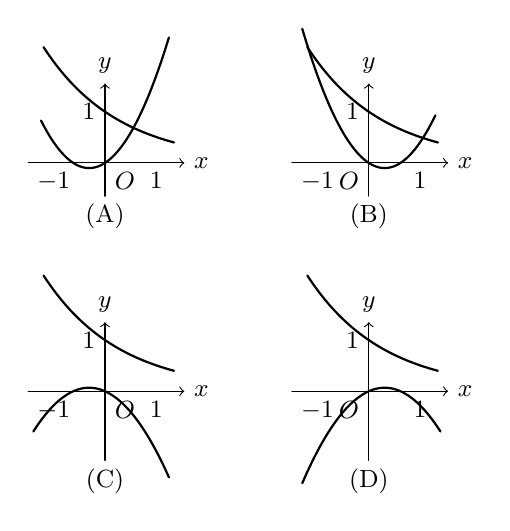
\begin{tikzpicture}[x=.65cm,y=.65cm,font=\small,line cap=round,line join=round]
  \begin{scope}
    \draw[->] (-1.5,0)--(1.55,0) node[right] {$x$};
    \draw[->] (0,-.65)--(0,1.55) node[above] {$y$};
    \draw[thick,domain=-1.25:1.25,samples=60,variable=\x] plot (\x,{1.05*\x*(\x+.62)});
    \draw[thick,domain=-1.2:1.35,samples=60,variable=\x] plot (\x,{exp(-.68*\x)});
    \node[below] at (-1,0) {$-1$}; \node[below right] at (0,0) {$O$}; \node[below] at (1,0) {$1$};
    \node[left] at (0,1) {$1$}; \node at (0,-1.05) {(A)};
  \end{scope}
  \begin{scope}[xshift=3.35cm]
    \draw[->] (-1.5,0)--(1.55,0) node[right] {$x$};
    \draw[->] (0,-.65)--(0,1.55) node[above] {$y$};
    \draw[thick,domain=-1.3:1.3,samples=60,variable=\x] plot (\x,{1.05*\x*(\x-.62)});
    \draw[thick,domain=-1.2:1.35,samples=60,variable=\x] plot (\x,{exp(-.68*\x)});
    \node[below] at (-1,0) {$-1$}; \node[below left] at (0,0) {$O$}; \node[below] at (1,0) {$1$};
    \node[left] at (0,1) {$1$}; \node at (0,-1.05) {(B)};
  \end{scope}
  \begin{scope}[yshift=-2.9cm]
    \draw[->] (-1.5,0)--(1.55,0) node[right] {$x$};
    \draw[->] (0,-1.35)--(0,1.35) node[above] {$y$};
    \draw[thick,domain=-1.4:1.25,samples=60,variable=\x] plot (\x,{-.72*\x*(\x+.62)});
    \draw[thick,domain=-1.2:1.35,samples=60,variable=\x] plot (\x,{exp(-.68*\x)});
    \node[below] at (-1,0) {$-1$}; \node[below right] at (0,0) {$O$}; \node[below] at (1,0) {$1$};
    \node[left] at (0,1) {$1$}; \node at (0,-1.75) {(C)};
  \end{scope}
  \begin{scope}[xshift=3.35cm,yshift=-2.9cm]
    \draw[->] (-1.5,0)--(1.55,0) node[right] {$x$};
    \draw[->] (0,-1.35)--(0,1.35) node[above] {$y$};
    \draw[thick,domain=-1.3:1.4,samples=60,variable=\x] plot (\x,{-.72*\x*(\x-.62)});
    \draw[thick,domain=-1.2:1.35,samples=60,variable=\x] plot (\x,{exp(-.68*\x)});
    \node[below] at (-1,0) {$-1$}; \node[below left] at (0,0) {$O$}; \node[below] at (1,0) {$1$};
    \node[left] at (0,1) {$1$}; \node at (0,-1.75) {(D)};
  \end{scope}
\end{tikzpicture}
\end{center}
\nopagebreak[4]
（A）　（B）　（C）　（D）

\end{question}
\gkpart{二、填空题（本大题满分 40 分，共 10 题，每空 4 分）}

只要求直接填写结果；每个空格填对得 4 分，否则一律得零分。

\begin{question}
\gkti{9}方程 $\log_2(9^x-5)=\log_2(3^x-2)+2$ 的解是 $x=\underline{\qquad\qquad}$。

\end{question}
\begin{question}
\gkti{10}函数

\nopagebreak[4]
\[
y=\dfrac{1}{\sqrt{\log_{1/2}(2-x)}}
\]

的定义域是 $\underline{\qquad\qquad}$。

\end{question}
\begin{question}
\gkti{11}方程 $\sin\dfrac{x}{2}=\dfrac13$ 在 $[\pi,2\pi]$ 上的解是 $x=\underline{\qquad\qquad}$。

\end{question}
\begin{question}
\gkti{12}函数 $y=x^{-2}\ (x<0)$ 的反函数是 $y=\underline{\qquad\qquad}$。

\end{question}
\begin{question}
\gkti{13}极坐标方程分别是 $\rho=\cos\theta$ 和 $\rho=\sin\theta$ 的两个圆的圆心距离是 $\underline{\qquad\qquad}$。

\end{question}
\begin{question}
\gkti{14}在 $(1+x)^6(1-x)^4$ 的展开式中，$x^3$ 的系数是 $\underline{\qquad\qquad}$（结果用数值表示）。

\end{question}
\gkpart{选做题：A1 组和 B1 组}

考生可从下列两组（A1 组和 B1 组）中选做一组试题，其中 A1 组适合非试点学校考生，B1 组适合试点学校考生。

\begin{question}
\gkti{15}

\textbf{A1 组：} 已知 $O(0,0)$ 和 $A(6,3)$ 两点，若点 $P$ 在直线 $OA$ 上，且 $\dfrac{OP}{PA}=\dfrac12$，又 $P$ 是线段 $OB$ 的中点，则点 $B$ 的坐标是 $\underline{\qquad\qquad}$。

\textbf{B1 组：} 已知 $\vec a+\vec b=2\vec i-8\vec j$，$\vec a-\vec b=-8\vec i+16\vec j$，那么 $\vec a\cdot\vec b=\underline{\qquad\qquad}$。

\begin{gktip}
\textbf{来源说明（A1）}：固定来源印作“点 $P$ 在直线 $OA$ 上”，题面照原文保留；该措辞及答案的核对结论见解析版。
\end{gktip}

\end{question}
\begin{question}
\gkti{16}

\textbf{A1 组：} 平移坐标轴将抛物线 $4x^2-8x+y+5=0$ 化为标准方程 $x'^2=ay'\ (a\ne0)$，则新坐标系的原点在原坐标系中的坐标是 $\underline{\qquad\qquad}$。

\Needspace{5\baselineskip}
\textbf{B1 组：}

\nopagebreak[4]
\[
\lim_{x\to2}\left(\dfrac{4}{x^2-4}-\dfrac{1}{x-2}\right)=\underline{\qquad\qquad}\text{。}
\]

\end{question}
\begin{question}
\gkti{17}有 8 本互不相同的书，其中数学书 3 本、外文书 2 本、其它书 3 本。

\textbf{A1 组：} 若将这些书排成一列放在书架上，则数学书恰好排在一起，外文书也恰好排在一起的排法共有 $\underline{\qquad\qquad}$ 种（结果用数值表示）。

\textbf{B1 组：} 若将这些书随机地排成一列放在书架上，则数学书恰好排在一起、外文书也恰好排在一起的概率为 $\underline{\qquad\qquad}$（结果用分数表示）。

\Needspace{0.4\textheight}
\end{question}
\begin{question}
\gkti{18}

\textbf{A1 组：} 如图，在正三角形 $ABC$ 中，$E,F$ 依次是 $AB,AC$ 的中点，$AD\perp BC$，$EH\perp BC$，$FG\perp BC$，$D,H,G$ 为垂足。若将正三角形 $ABC$ 绕 $AD$ 旋转一周所得圆锥的体积为 $V$，则其中由阴影部分所产生的旋转体的体积与 $V$ 的比值是 $\underline{\qquad\qquad}$。
\nopagebreak[4]
\begin{center}% 固定来源 PDF 印刷页 76 第 18 题 A1 组图形的矢量示意。
% 阴影对应上部 AEF 与两侧 BEH、FCG；仅绘结构，不补充比例条件。
\begin{tikzpicture}[scale=1.0,font=\small,line cap=round,line join=round]
  \coordinate (B) at (-2.2,0); \coordinate (C) at (2.2,0);
  \coordinate (A) at (0,3.4); \coordinate (D) at (0,0);
  \coordinate (E) at (-1.1,1.7); \coordinate (F) at (1.1,1.7);
  \coordinate (H) at (-1.1,0); \coordinate (G) at (1.1,0);
  \fill[pattern=north east lines] (A)--(E)--(F)--cycle;
  \fill[pattern=north east lines] (B)--(E)--(H)--cycle;
  \fill[pattern=north east lines] (F)--(C)--(G)--cycle;
  \draw[thick] (A)--(B)--(C)--cycle;
  \draw[thick] (E)--(F) (A)--(D) (E)--(H) (F)--(G);
  \draw (H) rectangle ++(.18,.18); \draw (G) rectangle ++(-.18,.18);
  \node[above] at (A) {$A$}; \node[below left] at (B) {$B$};
  \node[below right] at (C) {$C$}; \node[below] at (D) {$D$};
  \node[left] at (E) {$E$}; \node[right] at (F) {$F$};
  \node[below] at (H) {$H$}; \node[below] at (G) {$G$};
\end{tikzpicture}
\end{center}
\nopagebreak[4]
\Needspace{5\baselineskip}
\textbf{B1 组：} 若 $i$ 是虚数单位，计算

\nopagebreak[4]
\[
\dfrac{(1+\sqrt3i)^5}{16\sqrt2\left(\cos\dfrac{\pi}{6}-i\sin\dfrac{\pi}{6}\right)}=\underline{\qquad\qquad}\text{。}
\]

\end{question}
\gkpart{三、解答题（本大题满分 86 分，共 6 题，解答应写出必要步骤）}

\begin{question}
\gkti{19}\textbf{（本题满分 10 分）} 已知

\nopagebreak[4]
\[
\sin\left(\dfrac{\pi}{4}+\alpha\right)\sin\left(\dfrac{\pi}{4}-\alpha\right)=\dfrac16,
\qquad \alpha\in\left(\dfrac\pi2,\pi\right),
\]

求 $\sin4\alpha$ 的值。

\Needspace{0.4\textheight}
\end{question}
\begin{question}
\gkti{20}\textbf{（本题满分 10 分）} 在如图所示的直角坐标系中，一运动物体经过点 $A(0,9)$，其轨迹方程为 $y=ax^2+c\ (a<0)$，$D=(6,7)$ 为 $x$ 轴上的给定区间。

（1） （6 分） 为使物体落在 $D$ 内，求 $a$ 的取值范围；

（2） （4 分） 若物体运动时又经过点 $P(2,8.1)$，问它能否落在 $D$ 内？并说明理由。
\nopagebreak[4]
\begin{center}% 固定来源 PDF 印刷页 76 第 20 题坐标图的结构示意。
% D=(6,7) 为 x 轴开区间；曲线未按未知参数 a 定量绘制。
\begin{tikzpicture}[x=.78cm,y=.48cm,font=\small,line cap=round,line join=round]
  \draw[->] (-.45,0)--(8.2,0) node[right] {$x$};
  \draw[->] (0,-.45)--(0,10) node[above] {$y$};
  \draw[thick] (0,9)--(0,0);
  \fill (0,9) circle (1.4pt);
  \node[above left] at (0,9) {$A$}; \node[left] at (0,8.7) {$9$};
  \fill (2,8.1) circle (1.4pt); \node[above right] at (2,8.1) {$P$};
  \draw[densely dotted] (2,0)--(2,8.1);
  \draw[thick] (6,0)--(7,0); \fill[white] (6,0) circle (2.3pt); \fill[white] (7,0) circle (2.3pt);
  \draw (6,0) circle (2.3pt); \draw (7,0) circle (2.3pt);
  \node[below] at (6,0) {$6$}; \node[below] at (7,0) {$7$};
\end{tikzpicture}
\end{center}
\nopagebreak[4]
\Needspace{0.4\textheight}
\end{question}
\begin{question}
\gkti{21}\textbf{（本题满分 14 分）} 如图，在二面角 $\alpha-l-\beta$ 中，$A,B\in\alpha$，$C,D\in l$，$ABCD$ 为矩形。$P\in\beta$，$PA\perp\alpha$，且 $PA=AD$。$M,N$ 依次是 $AB,PC$ 的中点。

（1） （4 分） 求二面角 $\alpha-l-\beta$ 的大小；

（2） （5 分） 求证：$MN\perp AB$；

（3） （5 分） 求异面直线 $PA$ 与 $MN$ 所成角的大小。
\nopagebreak[4]
\begin{center}% 固定来源 PDF 印刷页 76 第 21 题空间图形的投影示意。
% 空间投影仅表示包含关系与平行/垂直结构，不作为比例图。
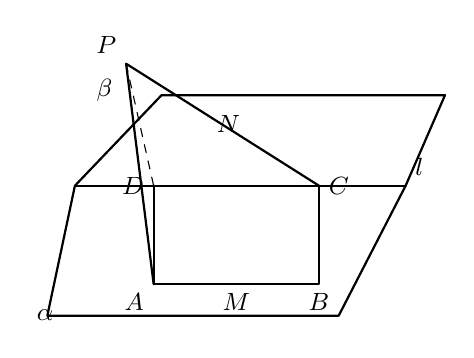
\begin{tikzpicture}[x=1cm,y=1cm,font=\small,line cap=round,line join=round]
  \coordinate (L) at (-.1,0); \coordinate (R) at (4.1,0);
  \coordinate (A1) at (.9,-1.25); \coordinate (B1) at (3.0,-1.25);
  \coordinate (D1) at (.9,0); \coordinate (C1) at (3.0,0);
  \coordinate (P) at (.55,1.55);
  \draw[thick] (L)--(R);
  \draw[thick] (L)--(1.0,1.15)--(4.6,1.15)--(R);
  \draw[thick] (L)--(-.45,-1.65)--(3.25,-1.65)--(R);
  \draw[thick] (A1)--(B1)--(C1)--(D1)--cycle;
  \draw[thick] (P)--(A1) (P)--(C1);
  \draw[dashed] (P)--(D1);
  \draw[thick] (A1)--(D1);
  \node[above left] at (P) {$P$}; \node[below left] at (A1) {$A$};
  \node[below] at (B1) {$B$}; \node[right] at (C1) {$C$}; \node[left] at (D1) {$D$};
  \node[below] at (1.95,-1.25) {$M$}; \node[above] at (1.85,.55) {$N$};
  \node[above right] at (R) {$l$}; \node[above left] at (.5,.95) {$\beta$};
  \node[below left] at (-.25,-1.45) {$\alpha$};
\end{tikzpicture}
\end{center}
\nopagebreak[4]
\end{question}
\begin{question}
\gkti{22}\textbf{（本题满分 16 分）} 本题有 A2、B2 两种选做版本；考生选做一组，其中 A2 组适合非试点学校考生，B2 组适合试点学校考生。

\textbf{A2 组：} 设 $z$ 是虚数，$w=z+\dfrac1z$ 是实数，且 $-1<w<2$。

（1） （6 分） 求 $|z|$ 的值及 $z$ 的实部的取值范围；

（2） （4 分） 设 $u=\dfrac{1-z}{1+z}$，求证：$u$ 为纯虚数；

（3） （6 分） 求 $w-u^2$ 的最小值。

\textbf{B2 组：} 已知 $A(-1,2)$ 为抛物线 $C:y=2x^2$ 上的点，直线 $l_1$ 过点 $A$，且与抛物线 $C$ 相切。直线 $l_2:x=a\ (a\ne-1)$ 交抛物线 $C$ 于点 $B$，交直线 $l_1$ 于点 $D$。

（1） （4 分） 求直线 $l_1$ 的方程；

（2） （5 分） 设 $\triangle ABD$ 的面积为 $S_1$，求 $|BD|$ 及 $S_1$ 的值；

（3） （7 分） 设由抛物线 $C$、直线 $l_1,l_2$ 所围成的图形面积为 $S_2$，求证：$S_1:S_2$ 的值为与 $a$ 无关的常数。

\Needspace{0.4\textheight}
\end{question}
\begin{question}
\gkti{23}\textbf{（本题满分 18 分）} 已知双曲线 $S$ 的两条渐近线过坐标原点，且与以点 $A(\sqrt2,0)$ 为圆心、$1$ 为半径的圆相切；双曲线 $S$ 的一个顶点 $A'$ 与点 $A$ 关于直线 $y=x$ 对称。设直线 $l$ 过点 $A$，斜率为 $k$。

（1） （4 分） 求双曲线 $S$ 的方程；

（2） （4 分） 当 $k=1$ 时，在双曲线 $S$ 的上支上求点 $B$，使其与直线 $l$ 的距离为 $\sqrt2$；

（3） （10 分） 当 $0\le k<1$ 时，若双曲线 $S$ 的上支上有且只有一个点 $B$ 到直线 $l$ 的距离为 $\sqrt2$，求斜率 $k$ 的值及相应点 $B$ 的坐标。
\nopagebreak[4]
\begin{center}% 固定来源 PDF 印刷页 77 第 23 题双曲线、渐近线及圆的矢量示意。
% 曲线和圆为结构示意，比例与切点位置不作为题设数据。
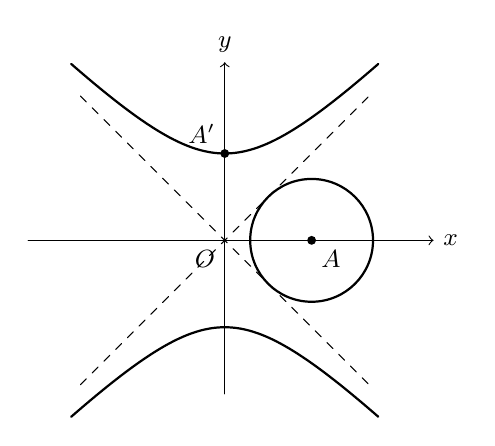
\begin{tikzpicture}[x=.78cm,y=.78cm,font=\small,line cap=round,line join=round]
  \draw[->] (-3.2,0)--(3.4,0) node[right] {$x$};
  \draw[->] (0,-2.5)--(0,2.9) node[above] {$y$};
  \draw[dashed] (-2.35,-2.35)--(2.35,2.35);
  \draw[dashed] (-2.35,2.35)--(2.35,-2.35);
  \draw[thick,domain=-2.5:2.5,samples=70,variable=\x]
    plot (\x,{sqrt(\x*\x+2)});
  \draw[thick,domain=-2.5:2.5,samples=70,variable=\x]
    plot (\x,{-sqrt(\x*\x+2)});
  \draw[thick] (1.414,0) circle (1);
  \fill (1.414,0) circle (1.6pt); \node[below right] at (1.414,0) {$A$};
  \fill (0,1.414) circle (1.6pt); \node[above left] at (0,1.414) {$A'$};
  \node[below left] at (0,0) {$O$};
\end{tikzpicture}
\end{center}
\nopagebreak[4]
\end{question}
\begin{question}
\gkti{24}\textbf{（本题满分 18 分）} 设 $A_n$ 为数列 $\{a_n\}$ 前 $n$ 项的和，

\nopagebreak[4]
\[
A_n=\dfrac32(a_n-1)\quad(n\in\mathbb N),
\]

数列 $\{b_n\}$ 的通项公式为 $b_n=4n+3\ (n\in\mathbb N)$。

（1） （5 分） 求数列 $\{a_n\}$ 的通项公式；

（2） （6 分） 若 $d\in\{a_1,a_2,a_3,\ldots\}\cap\{b_1,b_2,b_3,\ldots\}$，则称 $d$ 为数列 $\{a_n\}$ 与 $\{b_n\}$ 的公共项。将公共项按它们在原数列中的先后顺序排成新数列 $\{d_n\}$，证明数列 $\{d_n\}$ 的通项公式为 $d_n=3^{2n+1}\ (n\in\mathbb N)$；

（3） （7 分） 设数列 $\{d_n\}$ 中的第 $n$ 项是数列 $\{b_n\}$ 中的第 $r$ 项，$B_r$ 为数列 $\{b_n\}$ 前 $r$ 项的和，$D_n$ 为数列 $\{d_n\}$ 前 $n$ 项的和，$T_n=B_r-D_n$，求 $\displaystyle\lim_{n\to\infty}\dfrac{T_n}{(a_n)^4}$。

\end{question}